%!TEX root = ../thesis.tex

\cleardoublepage
\chapter{Evaluation}
\label{cha:evaluation}

This chapter reviews how the approach from the previous chapter was tested, and it discusses the observed results. The goal here is to explain the setup of the testbed, as well as the motivation behind the types of tests which were performed. Finally a discussion of the results and their implications will take place.


\section{Approach to Evaluating Performance}

In order to evaluate the success of the proposed approach, multipath scenarios will be emulated and investigated. Each setup will consist of two WAN connectors, and some number of emulated links going between them. The evaluations will be performed on a testbed consisted of four seperate host servers. Two of these servers will act as the originating and terminating WAN Connectors. One server will generate and measure traffic, in between the two WAn Connectors, a server will act as the link emulator. This architecture is shown in figure \ref{fig:testbed}

\begin{figure}[h]
    \centering
        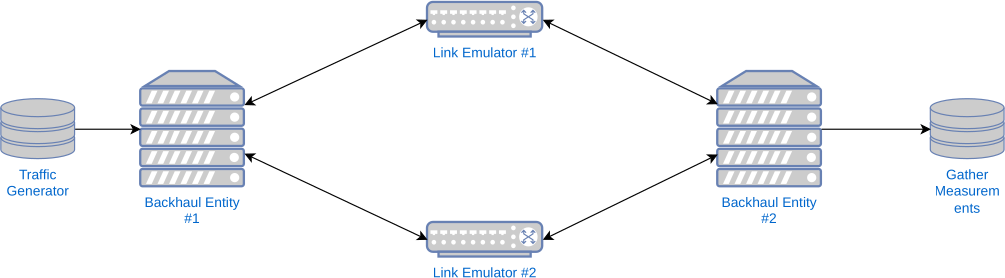
\includegraphics[width=0.66\textwidth]{fig/testbed.png}
        \caption{Testbed Setup}
        \label{fig:testbed}
\end{figure}

In figure \ref{fig:testbed}, the links between the servers are 10 GB ethernet cables. The hosts are connected as is shown. In the "traffic generator and measurer" two linux namespaces are used to separate the traffic generation and the measurement. The packets generated in one namespace are routed via the ethernet connection to the next host (the terminating or "edge" WAN Connector), because of the linux namespace they are not aware that their destination is technically the same host. The packets are then are backhauled by the WAN Connector over the emulated links in the next host, and via the terminating WAN Connector, back to the original host, but now in the "measurer" namespace.

The link emulation is done using the tc subsystem. First a root Heirarchical Token Bucket qdisc is established on the "downlink" and "uplink" interfaces (the ethernet cables between the WAN Connectors). In this case, the link emulation is performed before the outoing packet is queued on the ethernet cable, so that is also where the qdisc is placed. Secondly, the qdisc is given children classes, one class per link. This allows one to establish bandwidth caps for each emulated interface. Within these HTB classes the root qdisc is a netem qdisc. These allow the installation of link characteristics such as latency, packet loss, and jitter.

%In all of these scenarios the same traffic flows will be replayed. This traffic will contain different types of flows, with different QoS requirements. Before a new flow is started, the flow's requirements are sent to the WAN connector and it is either accepted or rejected. During the traffic replay, the delay, jitter, and reliability will be measured.

%All of these tests can be performed on the same testbed which will be set up as is shown in Figure \ref{fig:testbed}. The testbed architecture features a traffic generator, two WAN connectors, with a link emulator between them, and a measurement module to analyze performance. In practice the traffic generator and the test bench will be co-located on the same machine. The link emulator, and the WAN connectors are separate hosts, all interconnected over ethernet. The link emulation is done using the linux kernel's traffic control subsytem (TC). TC offers a network emulator (netem) queuing discipline (qdisc), which is able to emulate various link characteristics including delay, jitter, packet loss and packet re-ordering. Furthermore by combining the netem qdisc with a rate limiter, such as the Heirarchical Token Bucket (HTB) qdisc, a link can have its bandwidth limited. This allows one to emulate links with different latency, reliability and jitter, and with different maximum bandwidths.

In order to make the emulation more realistic, the netem qdiscs will periodically be adjusted, this allows one to degrade or improve links over time, for example by increasing the latency or packet loss in frequent intervals, up to a large value. It also more closely mimics the real-life behavior of WAN connections, which do experience changes in their characteristics over time.

For the purposes of evaluating the WAN connector, two initial series of experiments will be performed to isolate and investigate it's link switching capabilities. Firstly, purely latency based link selection will be investigated- a flow will be defined with specific latency requirements and then the emulated links will have their latency repeatedly changed. The WAN connector should then switch the flow to a different path. The same will be done once with packet loss. In the expriments with packet loss the WAN connector will have to choose between switching the flow to a different connection or duplicating it. During the duplication experiment, the application behind the flow should not receive any duplicate packets.

In order to simulate realistic scenarios these experiments will also be repeated with heavy background traffic which saturates the link's capabilites.


\section{Latency Based Path Switching}

For this scenario four links are emulated. The emulated links are based on simulation data from LEO satellites gathered using the SCNE simulator \footnote{https://connectivity.esa.int/projects/scne}. During the emulation, the simulation data is used to adjust the tc netem qdisc on the "link emulator" machine periodically. Because the SCNE simulator provides data over a 24 hour period, in 10 second intervals, the simulation data is "sped up". That is the emulation is changed each second, based on the next datapoint from the simulation. This means the 24 hour window can be run over a 2 hours test. Since real links are usually steadier and less volatile than the sped up emulation one can expect results in a real situation to be better.

In the experiment 100 packets are sent per second across each link, as well as 100 packets per second from the traffic generator, through the WAN Connector. This is done to have a comparison between the performance of the WAN Connector and the baseline performance level, which would be the best performing link. In any scenario the minimum acceptable performance of a path switching appliaction would be to provide a better performance than the best single link. Otherwise it would be better to just select the best link, and not use the application at all.

\subsection{Accuracy of the Emulation}

Figure \ref{fig:sim_vs_em} shows the comparison between the data observed in the emulation, and the simulation. The "emulated data" in the graphic is taken from the packet flows running over the individual links. The "simulation data" comes from the values recorded during the simulation. Since the emulation data is collected at a rate of 100 packets per second, and runs at 10 times the speed of the simulation, there are 10 times as many data points. This explains why the emulation data appears blurrier.

\begin{figure}[h]
    \centering
        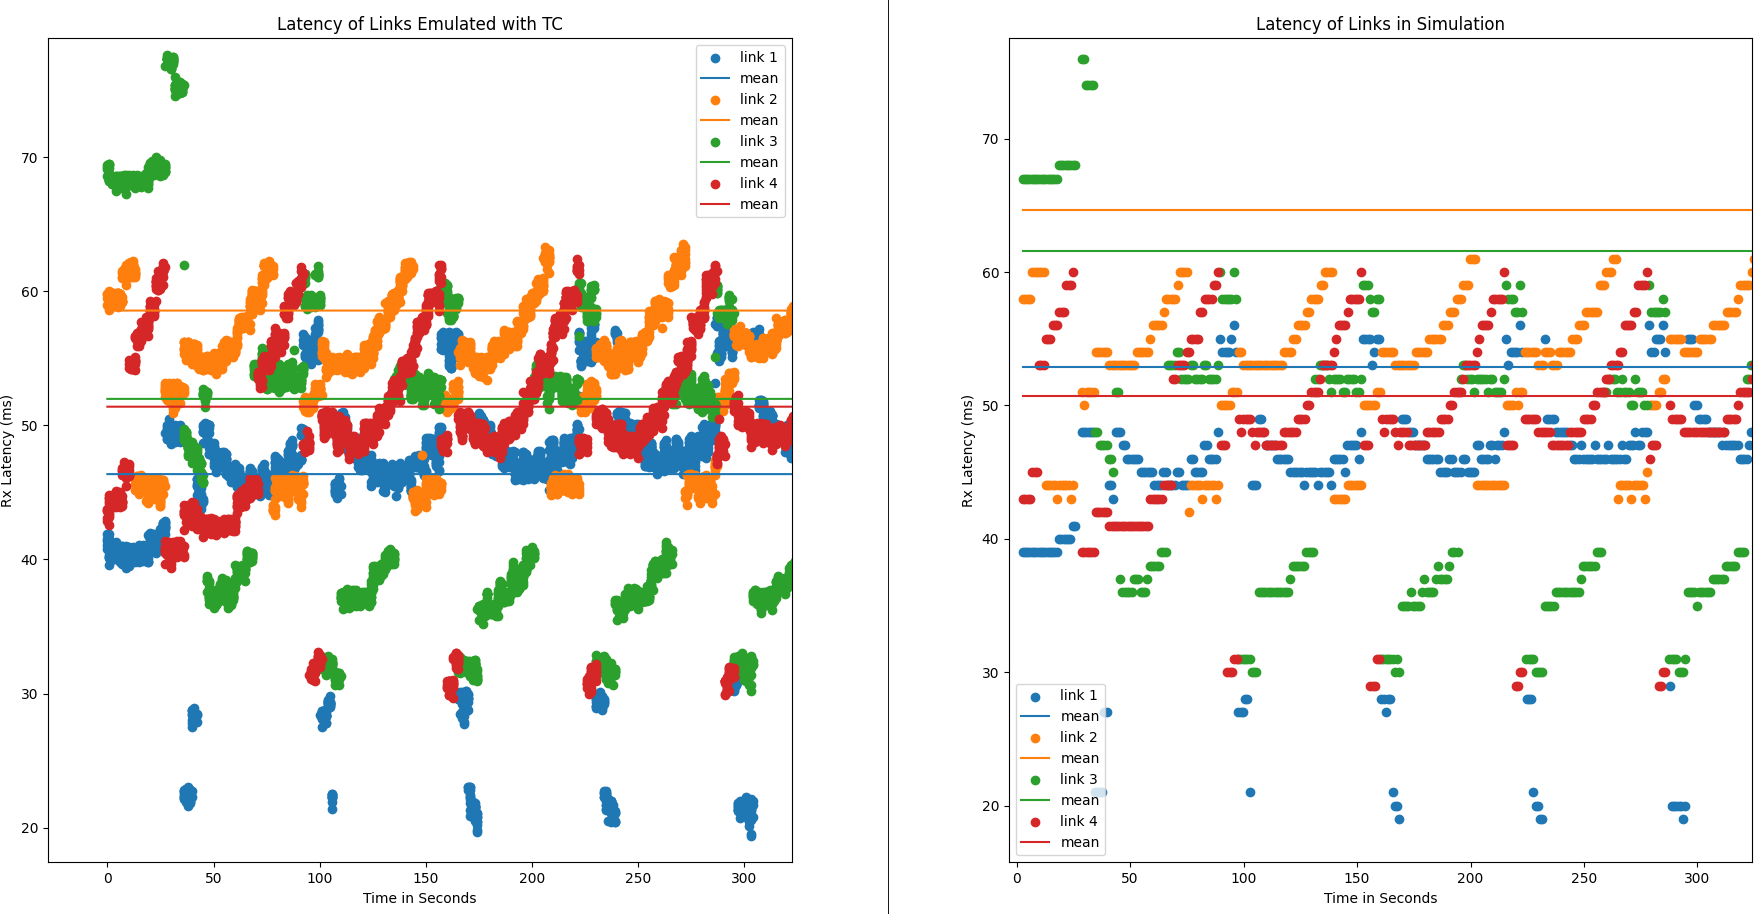
\includegraphics[height=0.66\textwidth,width=\textwidth]{fig/sim_vs_em_compariso.png}
        \caption{Accuracy of the Emulation}
        \label{fig:sim_vs_em}
\end{figure}

As the figure shows,  the latencies measured in the testbed mirror those recorded in the simulation, and serve to show that the emulation works, and is able to replicate the changing characteristics of the links during the simulation.

\subsection{Performance Compared to Single Links}

For the latency analysis a flow is defined in the WAN Connector with a minimum round trip time (RTT) of 56 milliseconds. This value is chosen because it is the mean of the mean values of the latencies of the four links in the simulation. The packets being matched 

\begin{figure}[h]
    \centering
        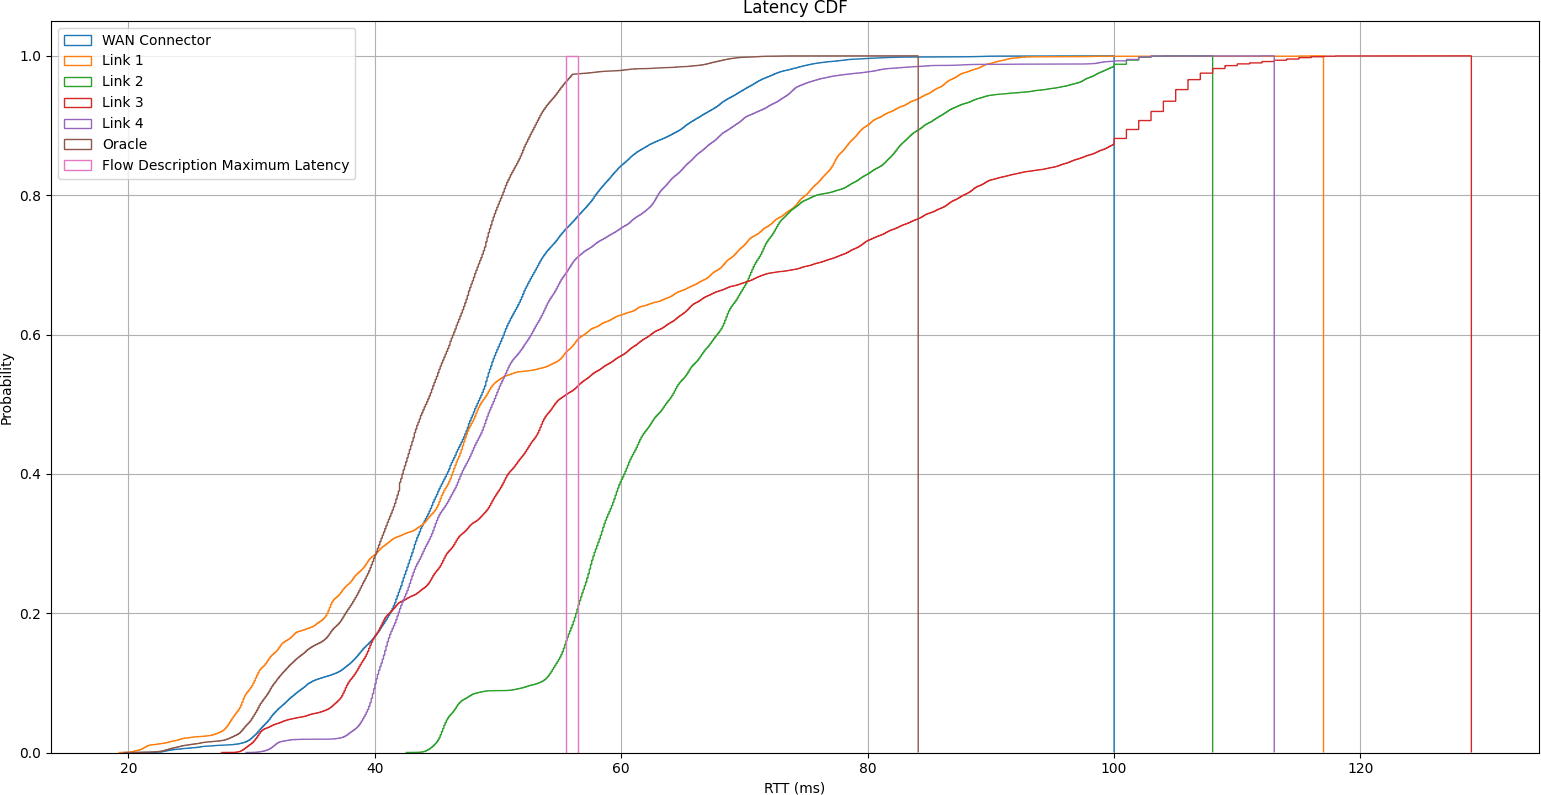
\includegraphics[height=0.66\textwidth,width=\textwidth]{fig/latency_cdf1.png}
        \caption{Cumulative Distribution of the Latencies}
        \label{fig:latency_cdf1}
\end{figure}

\begin{figure}[h]
    \centering
        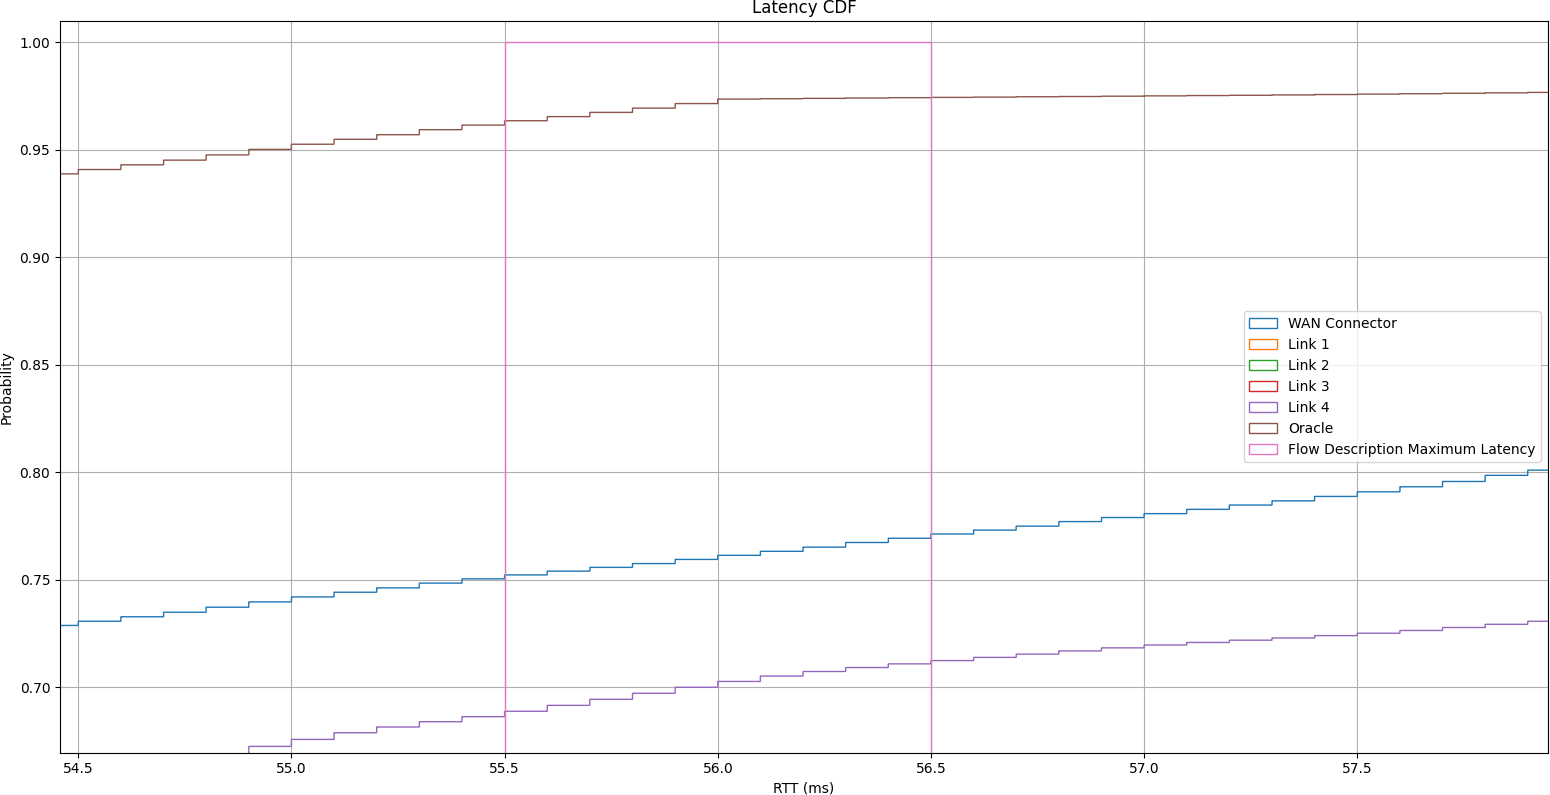
\includegraphics[height=0.66\textwidth,width=\textwidth]{fig/latency_cdf1_super_zoomed_in.png}
        \caption{Closeup of the Previous Figure}
        \label{fig:latency_cdf1_super_zoomed_in}
\end{figure}

The graphics \ref{fig:latency_cdf1} and \ref{fig:latency_cdf1_super_zoomed_in} show a cumulative distribution of the different latencies experienced by the packet flows running over the individual links and the WAN Connector, as well as the performance of the Oracle approach. The Oracle results are purely theoretical. For each packet, it is able to select the best link to forward on, based on that links future characteristics. This approach is calculated by comparing each packet sent by the WAN Connector with the latency that packet \textit{would} experience on any given link and if the latency of the WAN Connector's link would be greater than the minimum value (56 ms), selecting a different link (if one exits) which would have a lower latency. The Oracle approach provides an upper bound on the best possible performance. In practice it is not possible, of course, because it has knowledge of the future. But nonetheless it provides a very valuable comparison.

The results in the figures show that the WAN Connector is able to achieve a superior performance to any of the individual links on their own. This was the baseline requirement and it is important that it is able to achieve this. However the performance does not significantly improve on the next best link, which is is able to achieve the minimum required latency 72\% of the time, while the WAN Connector does so 77.5\% of the time. This pales in comparison to the Oracle approach which shows that in theory one could have maintained the minimum latency required by the flow in 95\% of the cases. This means the WAN Connector's performance is only 80\% optimal.

\subsection{Latency Performance Under Load and the Importance of Traffic Shaping}

During this experiment, the same 100 packet per second flow from before is repeated, but background traffic is added. An iperf3 test is run across the WAN Connector at the same time as the latency critical flow, and it is given the same latency requirements, so that the WAN Connector always schedules both flows to the same link. This ensures that whatever link is on will be saturated. Latency performance during congestion and close to congested scenarios is a crucial element of a deterministic backhaul solution. The WAN Connector's control plane only makes decision about which link to forward on- it does not perform load balancing or prioritization. The data plane does not do this either, it implement a purely First In First Out (FIFO) approach to packet queueing. This is done because the burden of implementing an appropriate packet shaper, in addition to the other multipath calculations, is too significant for the purposes of this thesis, and because very powerful traffic shaping implementations, which are easy to integrate into this solution, already exist.

\begin{figure}[h]
    \centering
        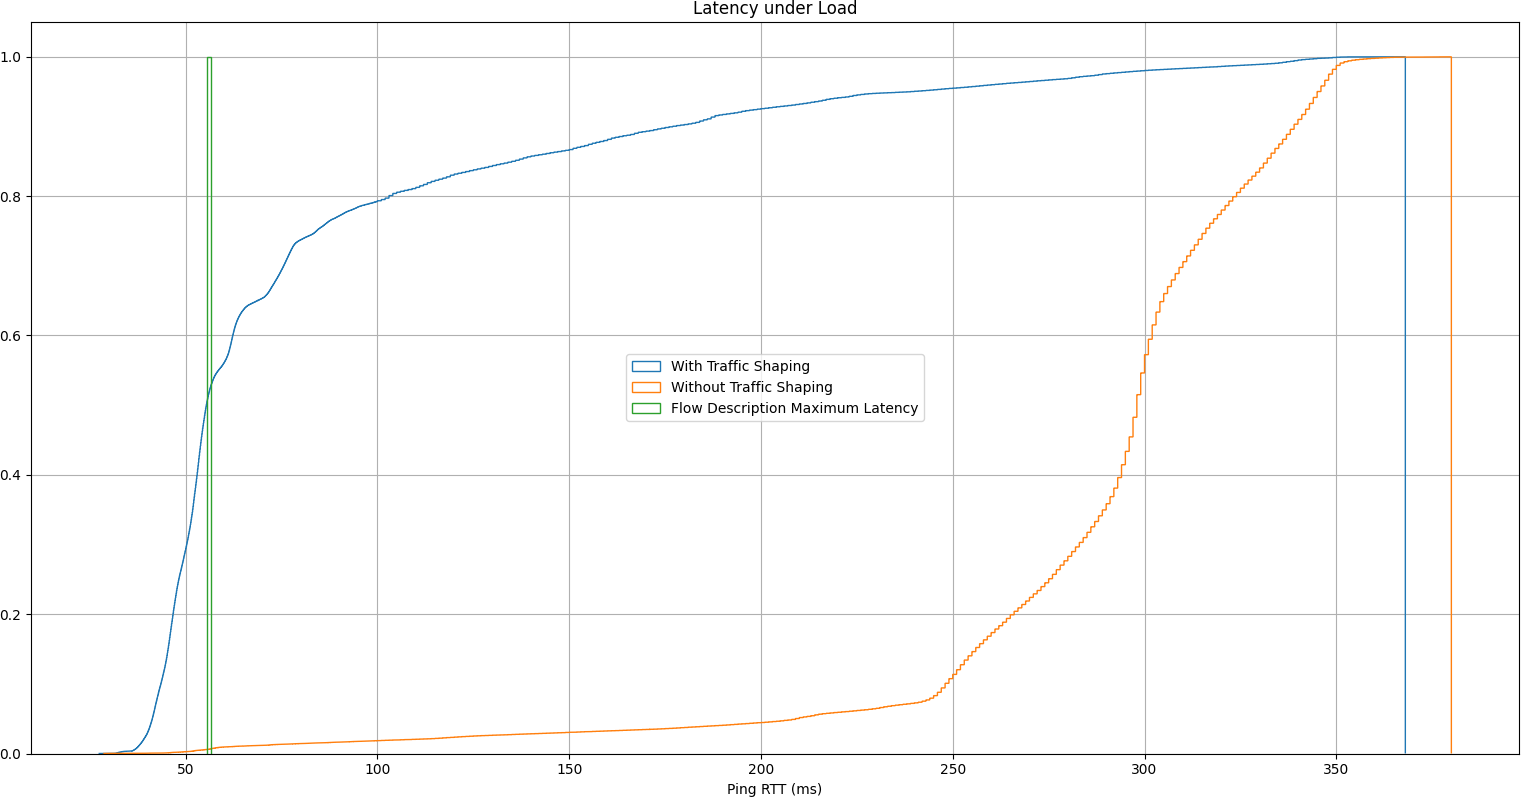
\includegraphics[height=0.66\textwidth,width=\textwidth]{fig/rrul_cdf.png}
        \caption{Latency with Background Traffic}
        \label{fig:rrul_cdf}
\end{figure}

The figure \ref{fig:rrul_cdf} neatly demonstrates why traffic shaping is an essential element of any deterministic network. In the case in which there is no traffic shaper the latency critical flow experiences significant additional latency due to the network being overloaded. The TCP algorithm fills the link's capacity, and the latency critical packets spend too much time buffering and arrive late. It should be noted that the WAN Connector's performance with the traffic shaper is worse than in the previous scenario, where there was no background traffic, and only 50\% of the packets are under the required latency of the critical flow. However the approach without the traffic shaping is at just 1\%.

\section{Reliability Based Path Switching}

In the next scenario, to analyze the ability of the WAN Connector to achieve the required reliability of a given flow, the same latency critical flows from before are run over the WAN Connector and the four outgoing links. However this time instead of varying the latency, the packet loss ratio of the link is change. The simulation's results are used once again. However since the simulation does not provide packet loss on a per second basis, the latencies of all the different links in the simulation are used. For the emulation, these 51 values are looped over in 10 second increments. Each link is given a shuffled set of these 51 values. This means that the cumulative value of the packet loss experienced by all of the links is the same (2\%), but the instantaneous values will differ. To appropriately analyze this scenario the flow being backhauled over the WAN Connector is given a reliability threshold of 0.1\% this is because in this scenario, where the existing links all provide an average of 2\% reliability, it becomes necessary to duplicate at some points, in order to achieve the required reliability. 

\begin{figure}[h]
    \centering
        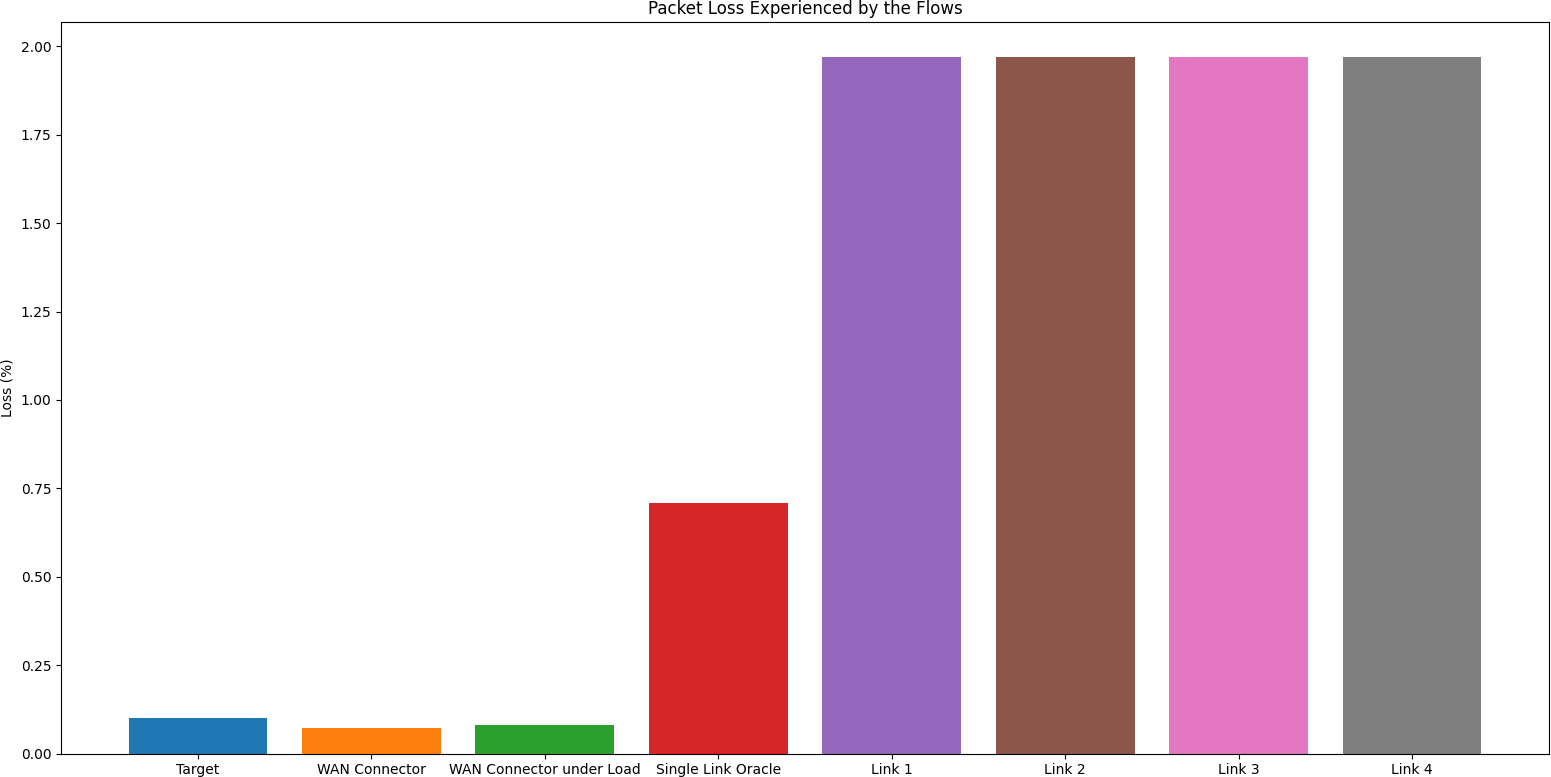
\includegraphics[height=0.66\textwidth,width=\textwidth]{fig/loss_bars1.png}
        \caption{Reliability}
        \label{fig:loss_bars1}
\end{figure}

For the analysis of the performance this time the Oracle approach is defined as choosing, before forwarding any packet, the link with the lowest packet loss ratio. But, crucially, the Oracle is not allowed to duplicate flows across different links. This explains why in figure \ref{fig:loss_bars1} the Oracle is outperformed by the WAN Connector. Indeed, as the graphic shows, it is not possible to achieve the critical flow's required reliability with any of the available links, nor with the Oracle approach. But the WAN Connector is able to achieve it. This speaks to the potency of the flow duplication approach, which is made possible in the optimization equation used to decided on which flows to forward.
































